\documentclass{article}
\usepackage{graphicx}
\usepackage{amsmath}
\usepackage{algorithm}
\usepackage[noend]{algpseudocode}
\usepackage{subcaption}
\usepackage{caption}
\usepackage[margin=0.6in]{geometry}

\makeatletter
\def\BState{\State\hskip-\ALG@thistlm}
\makeatother

\title{Feature Selection and Classification Methods}
\author{Derek Jones}


\begin{document}
\maketitle

\begin{center}
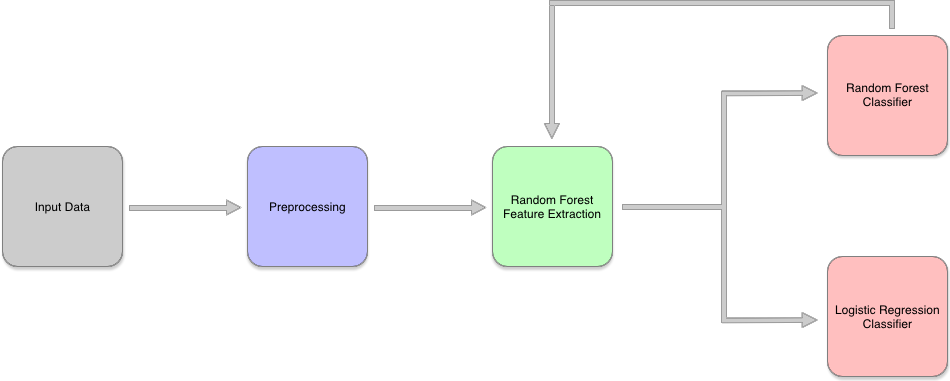
\includegraphics[scale=0.4]{/Users/derekjones2025/workspace/protein_binding/paper/figures/workflow_graphic.png}
\end{center}

\begin{abstract}
The following is a brief summary of the methods used in the prediction of active versus decoy drug-protein bindings for the full set of 26 protein kinases. 
\end{abstract}

\section{Preprocessing}
Before learning on the input data, it was necessary to preprocess the input. At least one column \textbf{(be more specific here)} contained missing values for a subset of the input training examples. One solution would be to simply drop any column with missing values, however it may be unwise to do this if the feature column has a small portion of missing values. (It has been shown that) Retaining the feature column and replacing the missing values via some strategy (here we use the mean of the non-empty values for all empty feature column values of the input training examples ) may improve classifier performance. 

It was also noted that a subset of feature columns contained relatively large values, increasing the computational burden of the learning algorithms given the size of our dataset. Here we normalize each feature column to unit vector length \textbf{(insert more details here)}.   

\section{Feature Selection}
The full dataset contains 5432 feature vectors per training example (~360,000). The ration of active versus decoy class labels in the set of trianing examples was approximately 1:50, with the decoys greatly outnumbering the actives in the training set. We use an 80/20 training testing split of our data. In the context of machine learning modles such as deep networks, adding more features to datasets with a large number of training examples may yield increasing returns due to the ability of deep networks to learn complex non linear relationships between feature maps and output labels. However this power requires the sacrifice of model interpretability, a property that is crucially important in the application field of bioinformatics. Due to this limitation as well as the difficulty that comes with training a network on a highly imbalanced dataset, it was decided that other less complicated models were more appropriate for our problem. 


A challenge in feature selection is finding a balance between computation time and the space of relationships one desires to consider to between the input feature maps and output labels. For example, variance thresholding (insert citation?) is a straightforward algorithm from which one may specify a minimum value of variance for which to tolerate the presence of a feature in the input, call this $\alpha$. The assumption here is that features that are \emph{near constant} in the input feature set are less informative than those features that vary by a greater amount. While this may be a valid quick and simple solution to the feature selection problem, it is impossible to capture any other relationship between feature value and class label, which the class label is not considered in the feature selection process of the variance thresholding method. For our problem this is a limitation that was not tolerable. Another option would be to use a \emph{LASSO} regression, aka Logistic Regression trained with an $L_{1}$ penalty term added to the loss function:
\begin{equation}
\mathcal{L}_{LASSO}(y,\bar{y}) = \mathcal{L}(y,\bar{y})+ \lambda \sum | ~ \theta  ~ |
\end{equation} 
The $L_{1}$ penalty term encourages the machine learning model to learn a set of weights for the input feature vectors that is sparse and may contain near and or absolute 0 entries. The weights obtained from adding this term to the loss function can be used to remove features that are not informative in the prediction of the target label. However one must take more care in using the LASSO regression as a feature selection method as it is possible that the model simply assigns weight 0 to all but 1 or a subset of weights for problems in which the negative and positive class values do not differ greatly in certain feature values. An alternative to LASSO regression is to take bootstrap samples from the trianing set and train LASSO regression models on each, then select a set of features that tend to not have 0 or small coefficient values (insert stability selection citation). However Randomized LASSO can be computationally expensive for problems with large input feature spaces, and large numbers of training examples, which makes the method impractical for our problem. 

% intro to random forests and their uses in classification and feature selection.
Random Forests \textbf{(citation, 2001)} are known to produce robust classifiers that are less prone to overfitting than ordinary decision trees or neural networks. For a brief review, a random forest is an ensemble method that uses a set of decision trees that are trained on samples from the training data (we use bootstrap sampling), each on a subset of the full feature set \textbf{(provide details on the number, sklearn has this)}. Upon test time, the input training example is fed to each tree and the mode across the decision trees (most common label) is taken to be the predicted output label of the forest. By using subsets of the data and feature space, random forests are much quicker to train than a deep neural network and other linear models such as logistic regression, and come with the benefit of being robust classifiers that tend to generalize as well or better as the aforementioned methods. From training a random forest, one can compute feature importances by the following equation:
\begin{equation}
Imp(X_{m}) = \frac{1}{N_{T}}\sum_{T}\sum_{t \in T:v(s_{t}) = X_{m}}p(t)\Delta i(s_t,t)
\end{equation}

Alternative to both variance thresholding, which does not allow for the relationship between feature values and target labels to be considered in the feature selection process, and randomized LASSO which requires large computational resources to train multiple logistic regression on a number of bootstrap samples from the dataset, the feature importances given by the random forest can be used instead. This method may be much quicker and possibly more informative than other feature selection methods. 

For our problem we make use of an iterative method to perform feature selection. Rather than simply training a random forest and extracting the relevant features from the input feature space, we use the output most important features of each previous step (defined to be the features whose importances are greater than the mean importance, i.e. importance greater than $1/n$) as the input space for the next step. We do this until a stopping criterion is achieved (decrease of metric of interest, f1-score, by greater than .001). We are able to reduce the input feature space by 2 orders of magnitude, from 5432 features to a set of 59 features, while retaining nearly the same performance across our metric of interest on each iteration of the evaluation step, in which we train and evaluate both a logistic regression and an additional random forest. A summary of the results are given in the next section.

%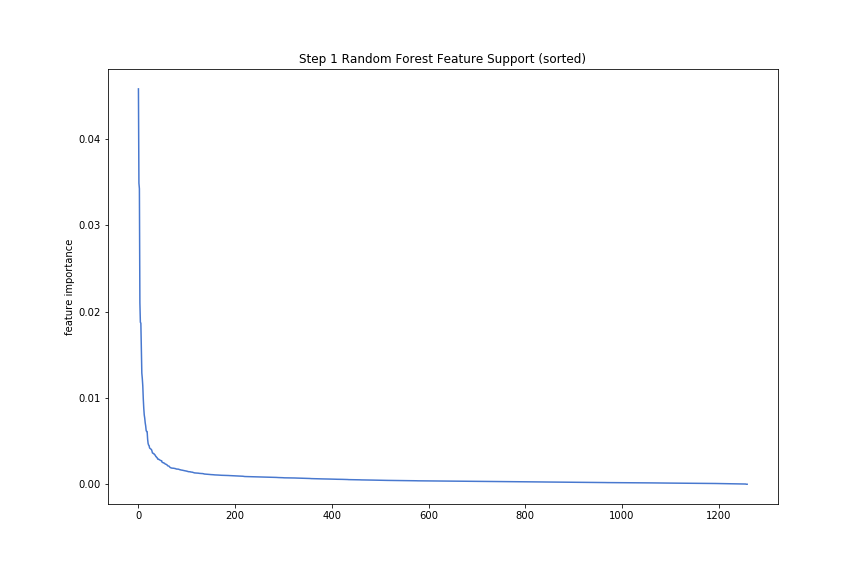
\includegraphics[scale=0.2]{/Users/derekjones2025/workspace/protein_binding/results/full_kinase_set/feature_importance_curve_step1.png}
%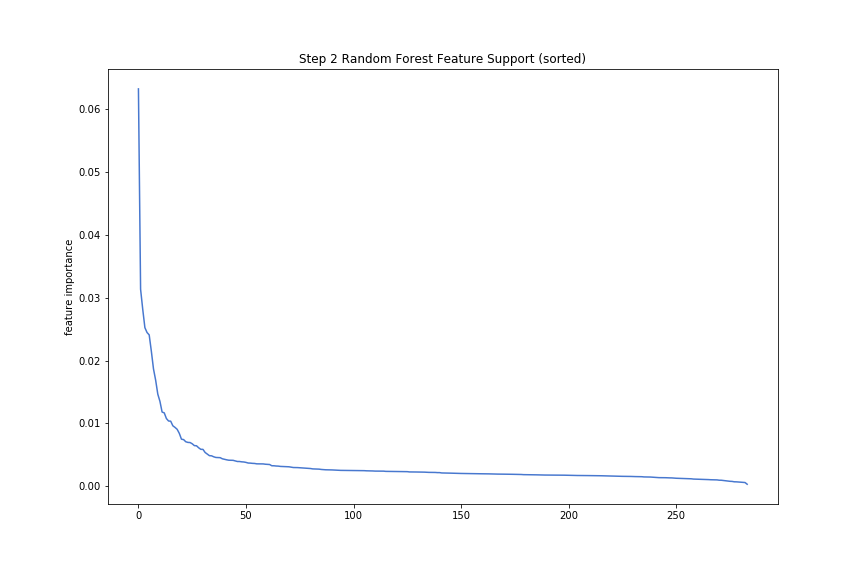
\includegraphics[scale=0.2]{/Users/derekjones2025/workspace/protein_binding/results/full_kinase_set/feature_importance_curve_step2.png}
%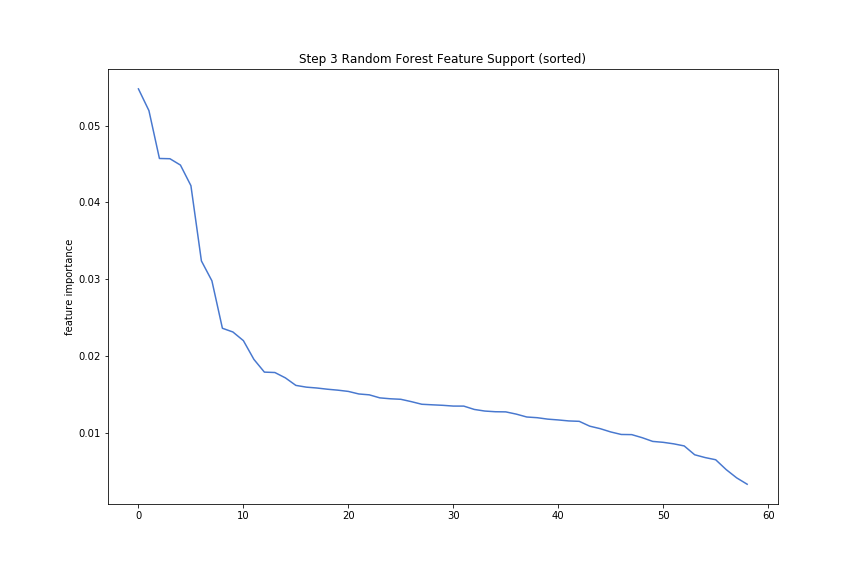
\includegraphics[scale=0.2]{/Users/derekjones2025/workspace/protein_binding/results/full_kinase_set/feature_importance_curve_step3.png}
%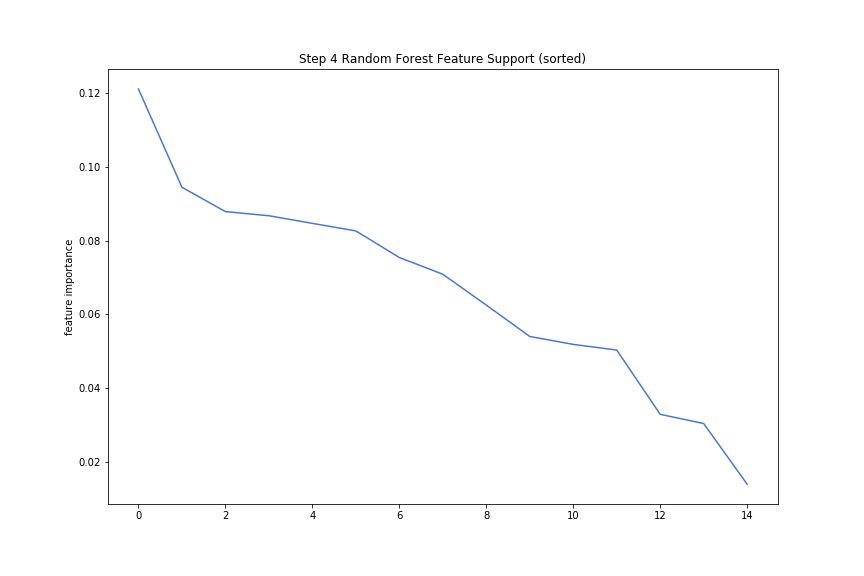
\includegraphics[scale=0.2]{/Users/derekjones2025/workspace/protein_binding/results/full_kinase_set/feature_importance_curve_step4.png}

\section{Classification Results}
\subsection{Experiment Details}
\begin{enumerate}
	\item input data (after preprocessing) partitioned into train test sets using an 80/20 stratified split. This was done in order to ensure the presence of positive labeled examples in the test set. (Try other splits?)
	\item  Model selection using randomized grid search. sampling from the distributions of hyperparameter values rather than trying an exhaustive search of all combinations of an input grid is more efficient and yields similar performance (possibly better, insert reference to bengio). 
	\item starting with 5432 features, a reduced set of (~1200) features are generated by extracting the feature importances from the forest, computing the mean importance ($1/n$), and removing all features that fall below the mean importance (could possibly try using different levels of confidence, one for each case of greater than or less than $1/n$).
	\item A random forest and logistic regression are trained on top of the reduced feature set (~1200). Confusion matrices as well as accuracy, f1-score, precision, and recall are computed for each classifier, the scores are broken down by class and given globally. 
	\item From the trained random forest, the feature importances are extracted via the same method as before
	\item These experiments were run using the experimental NERSC jupyter server on CORI at Berkeley Labs.
\end{enumerate}
In general, the classifier performance remains nearly the same across iterations suggesting that this method of feature selection is successful in ruling out extra information with marginal benefit to the classification power of the given method. 

The Random Forest tends to perform quite well on each iteration of reduced features along with a tendency to misclassify positive examples as negatives. This corresponds to labeling a drug as not binding to a protein. This may cause a hypothetical user to forego a promising candidate drug molecule.

The Logistic Regression performs better at correctly classifying positive training examples, however the method tends to misclassify negative training examples as positive. This may cause a hypothetical user to spend investment resources to develop a candidate drug molecule that does not in actuality inhibit the target receptor.


\begin{algorithm}
\caption{Iterative Selection Forest}\label{euclid}
\begin{algorithmic}[1]
\Procedure{MyProcedure}{}
\State $\textit{stringlen} \gets \text{length of }\textit{string}$
\State $i \gets \textit{patlen}$
\BState \emph{top}:
\If {$i > \textit{stringlen}$} \Return false
\EndIf
\State $j \gets \textit{patlen}$
\BState \emph{loop}:
\If {$\textit{string}(i) = \textit{path}(j)$}
\State $j \gets j-1$.
\State $i \gets i-1$.
\State \textbf{goto} \emph{loop}.
\State \textbf{close};
\EndIf
\State $i \gets i+\max(\textit{delta}_1(\textit{string}(i)),\textit{delta}_2(j))$.
\State \textbf{goto} \emph{top}.
\EndProcedure
\end{algorithmic}
\end{algorithm}


\subsection{Results: Classifier Metric Comparison}

\subsection{Results: Confusion Comparsion}
%\pagebreak
   
\begin{center}
\begin{figure}[htpb!]
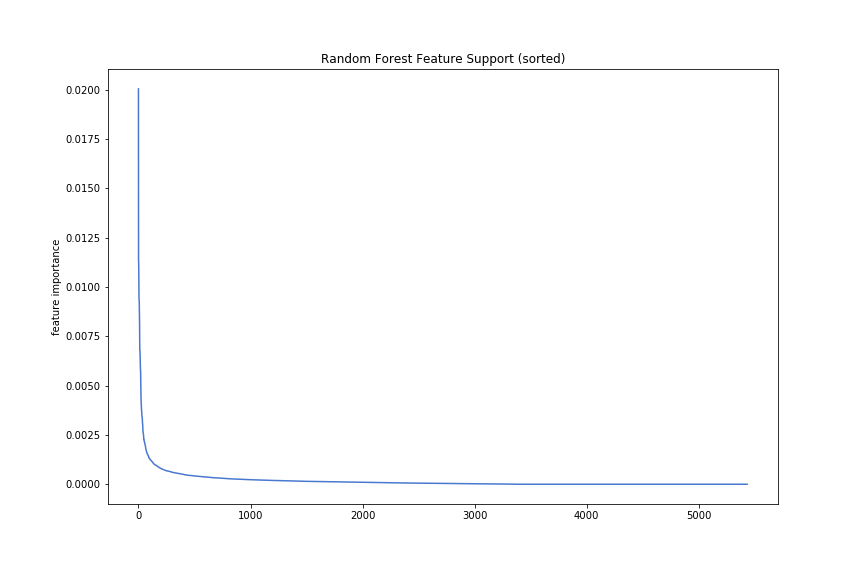
\includegraphics[scale=0.5, width=1\linewidth]{/Users/derekjones2025/workspace/protein_binding/results/full_kinase_set/feature_importance_curve_full_set.png}
\end{figure}
\end{center}

\begin{center}
\begin{figure}[htpb!]
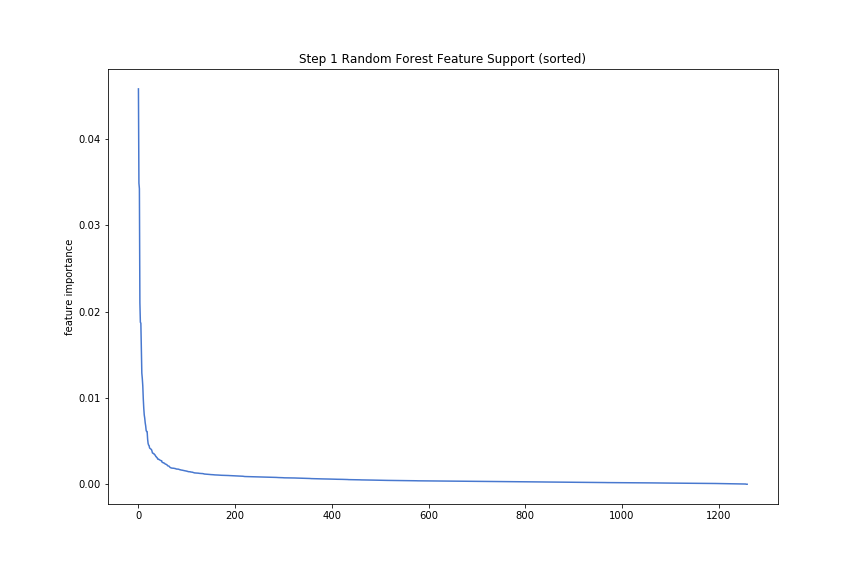
\includegraphics[scale=0.5, width=1\linewidth]{/Users/derekjones2025/workspace/protein_binding/results/full_kinase_set/feature_importance_curve_step1.png}
\end{figure}
\end{center}

\begin{center}
\begin{figure}[htpb!]
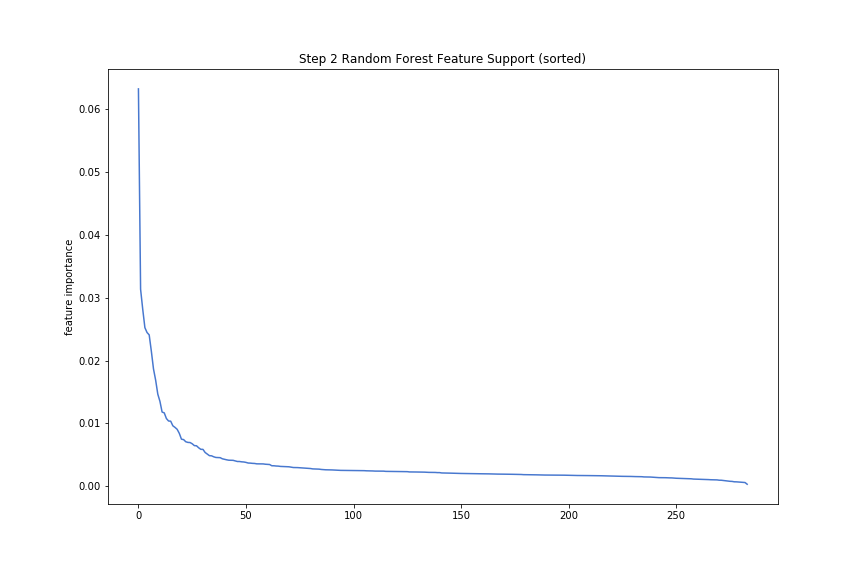
\includegraphics[scale=0.5, width=1\linewidth]{/Users/derekjones2025/workspace/protein_binding/results/full_kinase_set/feature_importance_curve_step2.png}
\end{figure}
\end{center}



\begin{figure}[htpb!]
%\centering
\begin{subfigure}{.5\textwidth}
%  \centering
  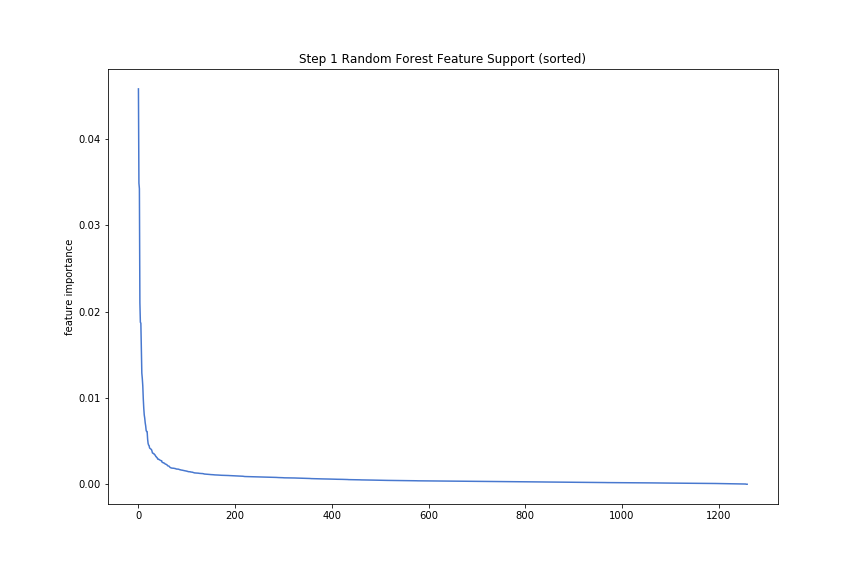
\includegraphics[width=1\linewidth]{/Users/derekjones2025/workspace/protein_binding/results/full_kinase_set/feature_importance_curve_step1.png}
  \caption*{$i=1$}
  \label{fig:sub1}
\end{subfigure}%
\begin{subfigure}{.5\textwidth}
%  \centering
  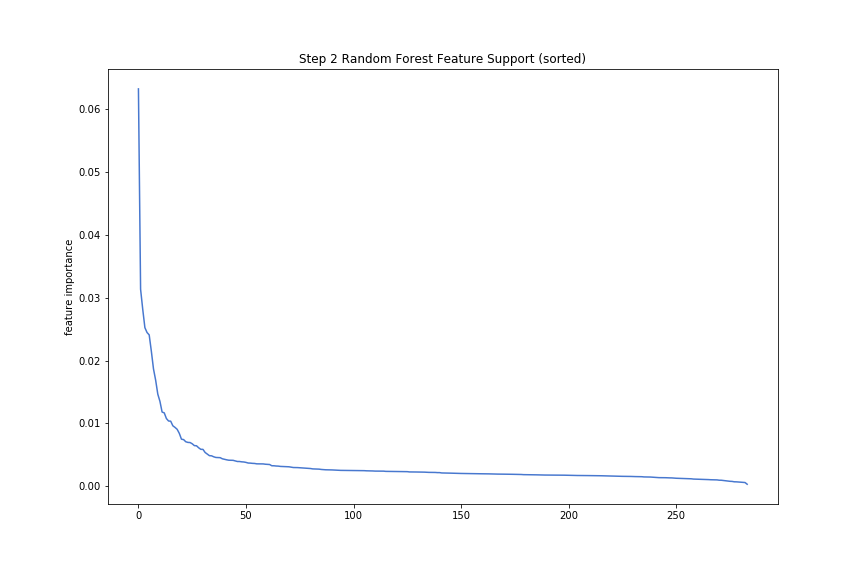
\includegraphics[width=1\linewidth]{/Users/derekjones2025/workspace/protein_binding/results/full_kinase_set/feature_importance_curve_step2.png}
  \caption*{$i=2$}
  \label{fig:sub2}
\end{subfigure}
%\caption*{$i=1$}
\label{fig:test}
\end{figure}



\begin{figure}[htpb!]
%\centering
\begin{subfigure}{.5\textwidth}
%  \centering
  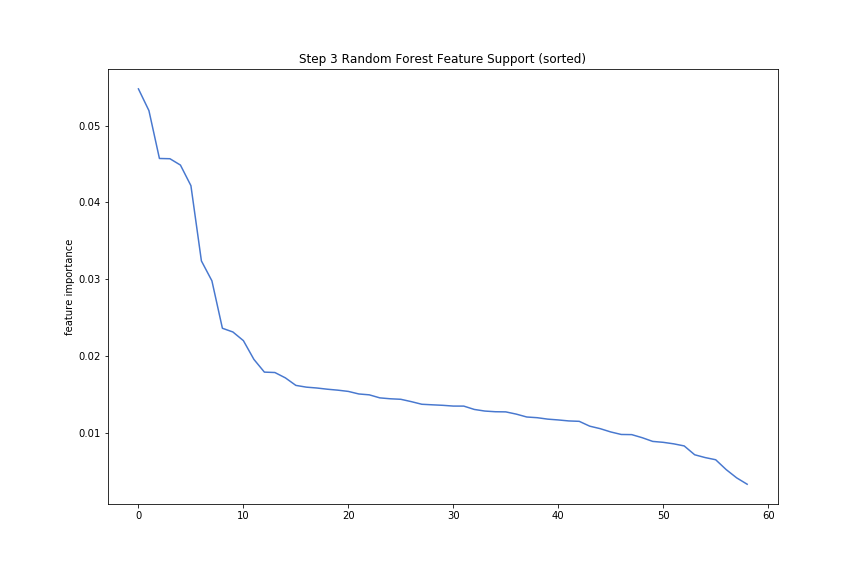
\includegraphics[width=1\linewidth]{/Users/derekjones2025/workspace/protein_binding/results/full_kinase_set/feature_importance_curve_step3.png}
  \caption*{$i=3$}
  \label{fig:sub1}
\end{subfigure}%
\begin{subfigure}{.5\textwidth}
%  \centering
  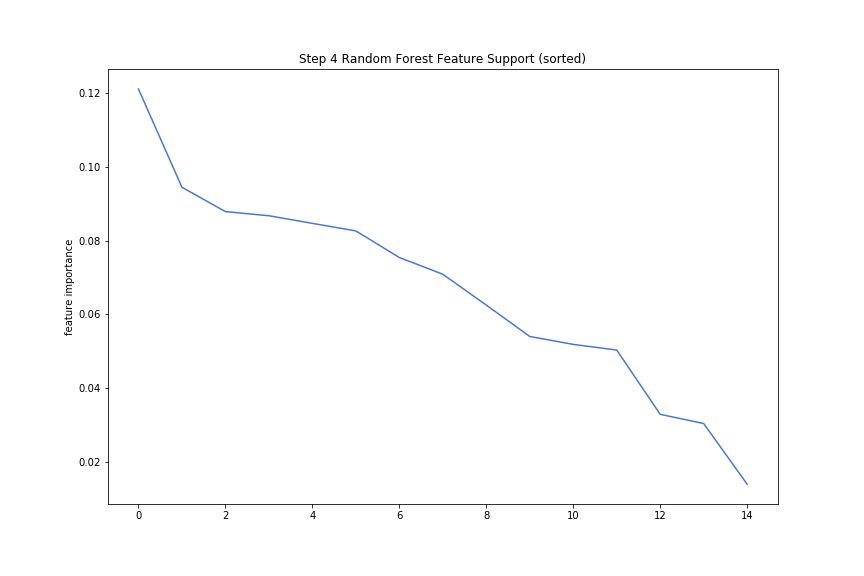
\includegraphics[width=1\linewidth]{/Users/derekjones2025/workspace/protein_binding/results/full_kinase_set/feature_importance_curve_step4.png}
  \caption*{$i=4$}
  \label{fig:sub2}
\end{subfigure}
%\caption*{$i=1$}
\label{fig:test}
\end{figure}




\begin{figure}[htpb!]
%\centering
\begin{subfigure}{.5\textwidth}
%  \centering
  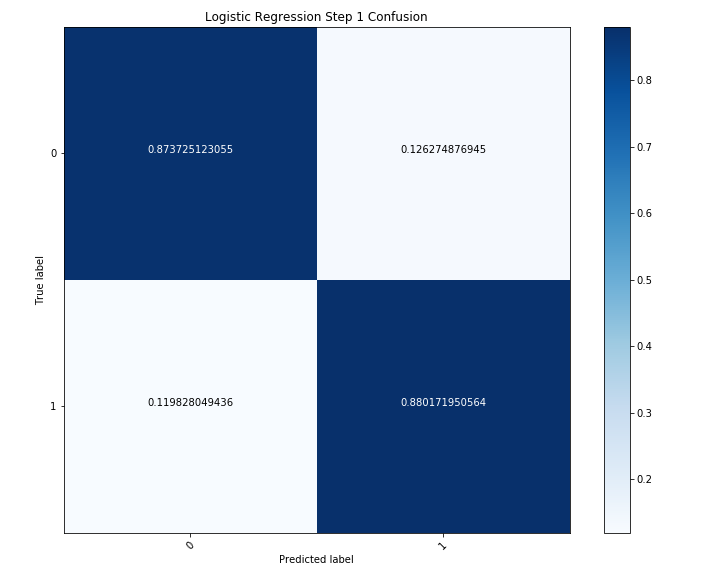
\includegraphics[width=1\linewidth]{/Users/derekjones2025/workspace/protein_binding/results/full_kinase_set/log_reg_step1_confusion.png}
  \caption{Logistic Regression}
  \label{fig:sub1}
\end{subfigure}%
\begin{subfigure}{.5\textwidth}
%  \centering
  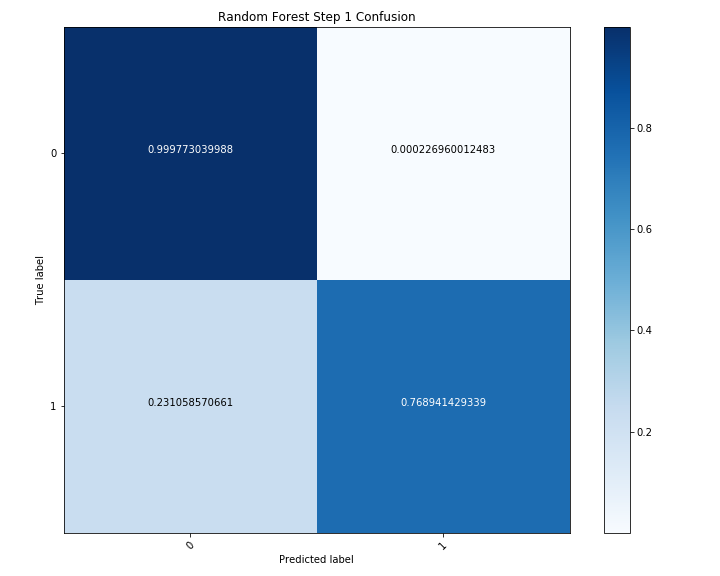
\includegraphics[width=1\linewidth]{/Users/derekjones2025/workspace/protein_binding/results/full_kinase_set/random_forest_step1_confusion.png}
  \caption{Random Forest}
  \label{fig:sub2}
\end{subfigure}
\caption*{$i=1$}
\label{fig:test}
\end{figure}


\begin{figure}[htpb!]
%\centering
\begin{subfigure}{.5\textwidth}
%  \centering
  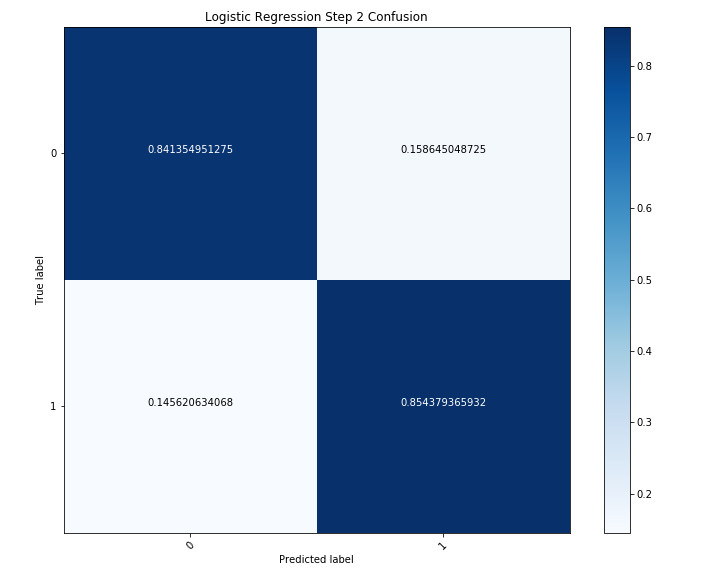
\includegraphics[width=1\linewidth]{/Users/derekjones2025/workspace/protein_binding/results/full_kinase_set/log_reg_step2_confusion.png}
  \caption{Logistic Regression}
  \label{fig:sub1}
\end{subfigure}%
\begin{subfigure}{.5\textwidth}
%  \centering
  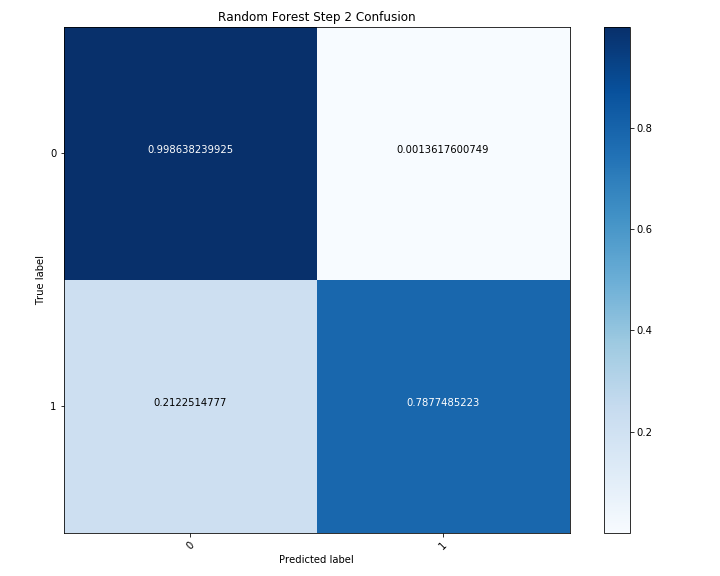
\includegraphics[width=1\linewidth]{/Users/derekjones2025/workspace/protein_binding/results/full_kinase_set/random_forest_step2_confusion.png}
  \caption{Random Forest}
  \label{fig:sub2}
\end{subfigure}
\caption*{$i=2$}
\label{fig:test}
\end{figure}



\begin{figure}[htpb!]
%\centering
\begin{subfigure}{.5\textwidth}
%  \centering
  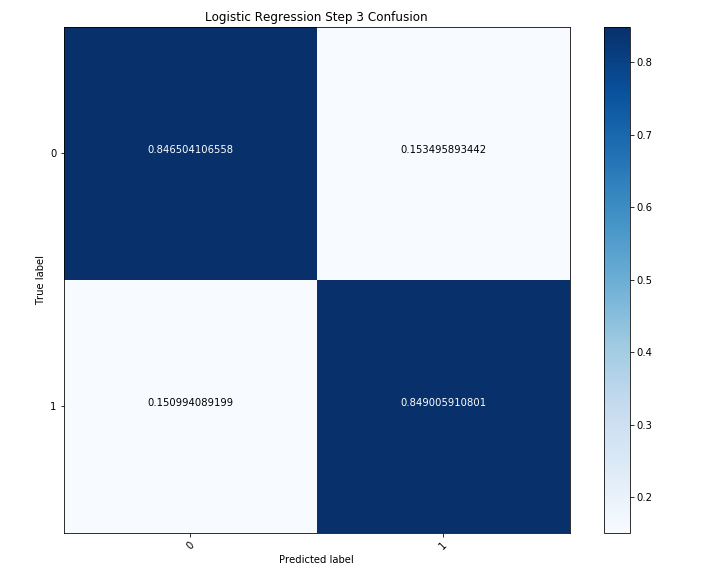
\includegraphics[width=1\linewidth]{/Users/derekjones2025/workspace/protein_binding/results/full_kinase_set/log_reg_step3_confusion.png}
  \caption{Logistic Regression}
  \label{fig:sub1}
\end{subfigure}%
\begin{subfigure}{.5\textwidth}
%  \centering
  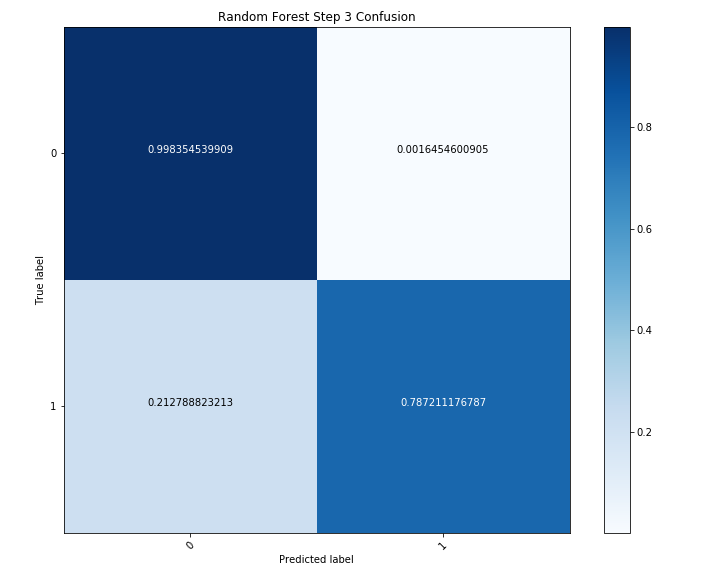
\includegraphics[width=1\linewidth]{/Users/derekjones2025/workspace/protein_binding/results/full_kinase_set/random_forest_step3_confusion.png}
  \caption{Random Forest}
  \label{fig:sub2}
\end{subfigure}
\caption*{$i=3$}
\label{fig:test}
\end{figure}


\begin{figure}[htpb!]
%\centering
\begin{subfigure}{.5\textwidth}
%  \centering
  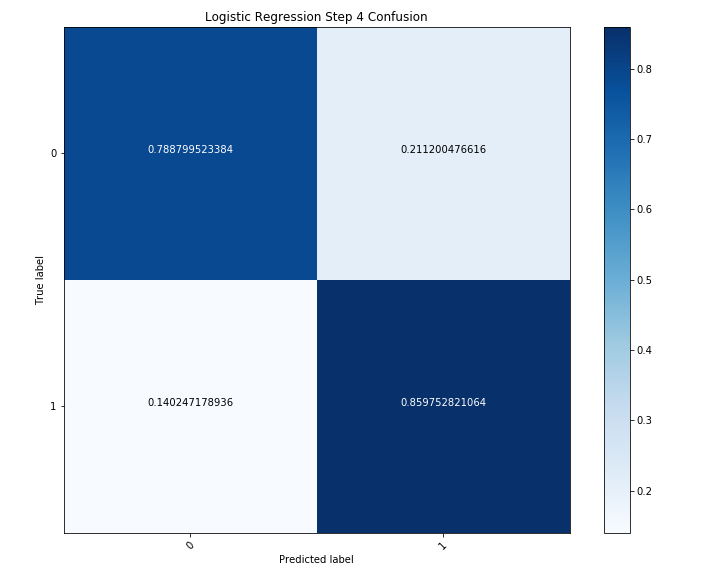
\includegraphics[width=1\linewidth]{/Users/derekjones2025/workspace/protein_binding/results/full_kinase_set/log_reg_step4_confusion.png}
  \caption{Logistic Regression}
  \label{fig:sub1}
\end{subfigure}%
\begin{subfigure}{.5\textwidth}
%  \centering
  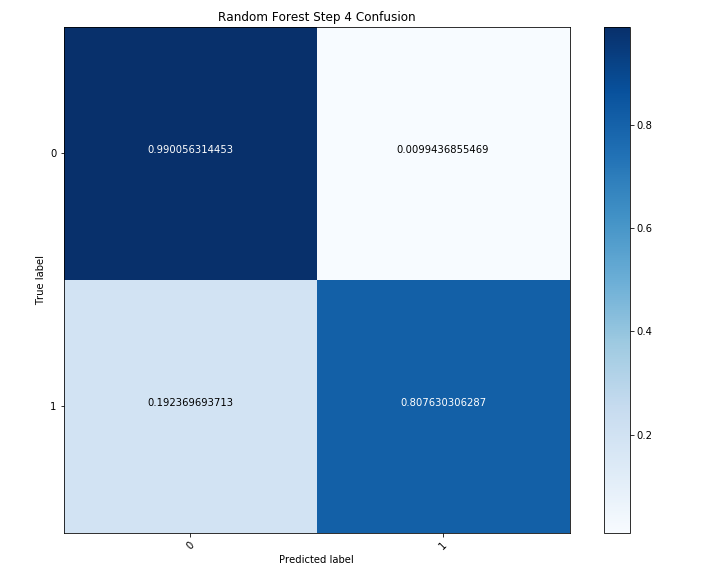
\includegraphics[width=1\linewidth]{/Users/derekjones2025/workspace/protein_binding/results/full_kinase_set/random_forest_step4_confusion.png}
  \caption{Random Forest}
  \label{fig:sub2}
\end{subfigure}
\caption*{$i=4$}
\label{fig:test}
\end{figure}

%\section{Classification}
%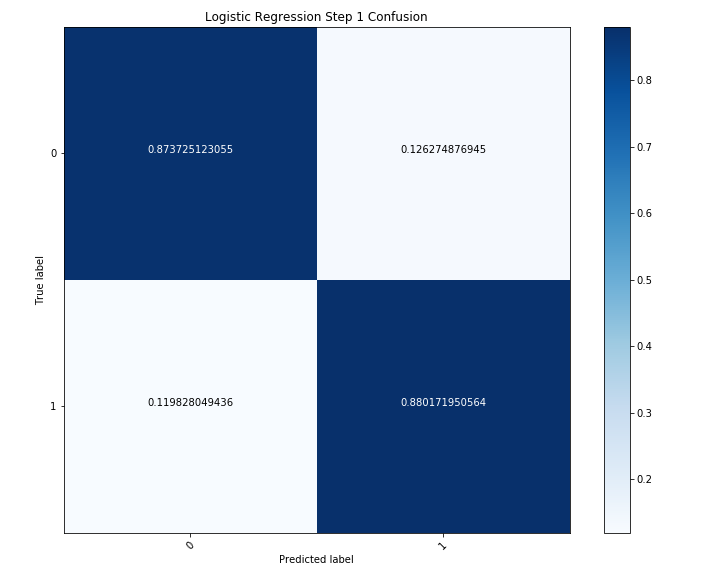
\includegraphics[scale=0.2]{/Users/derekjones2025/workspace/protein_binding/results/full_kinase_set/log_reg_step1_confusion.png}
%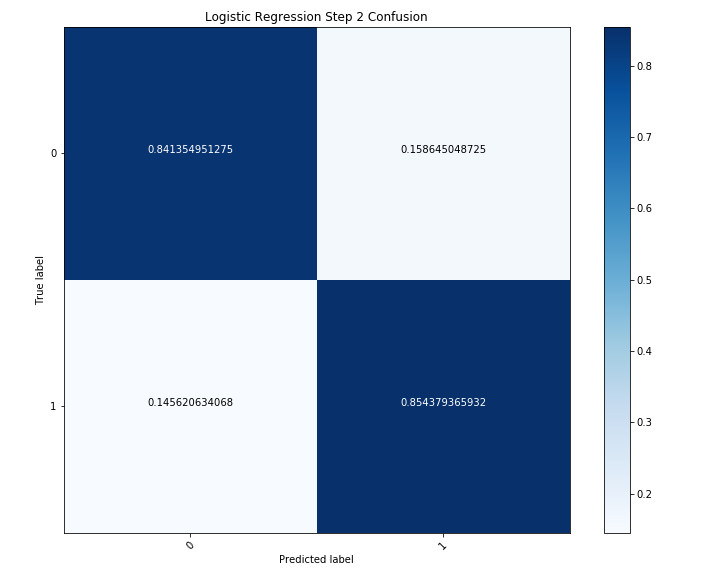
\includegraphics[scale=0.2]{/Users/derekjones2025/workspace/protein_binding/results/full_kinase_set/log_reg_step2_confusion.png}
%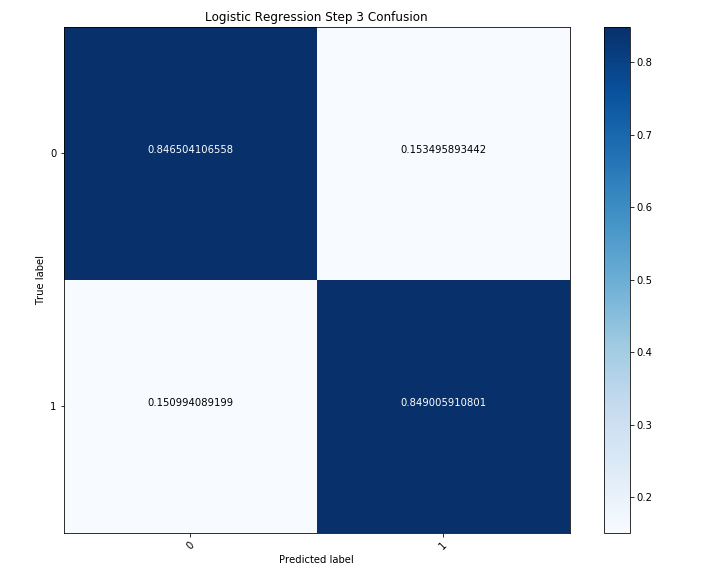
\includegraphics[scale=0.2]{/Users/derekjones2025/workspace/protein_binding/results/full_kinase_set/log_reg_step3_confusion.png}
%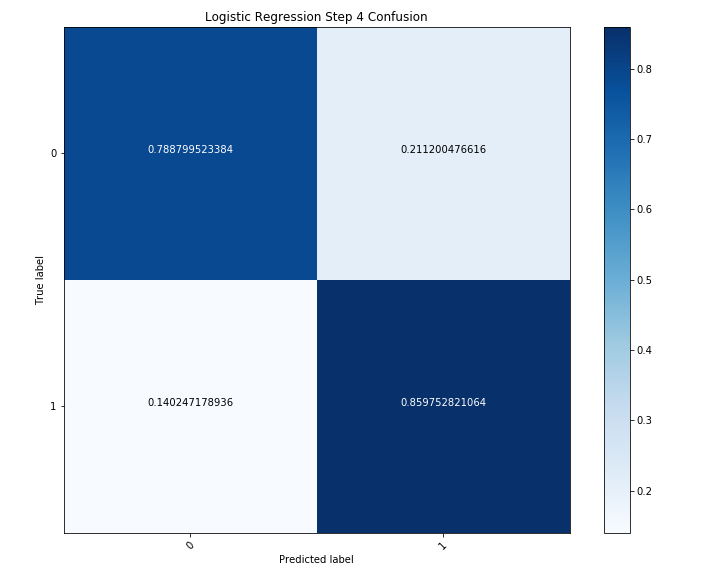
\includegraphics[scale=0.2]{/Users/derekjones2025/workspace/protein_binding/results/full_kinase_set/log_reg_step4_confusion.png}

%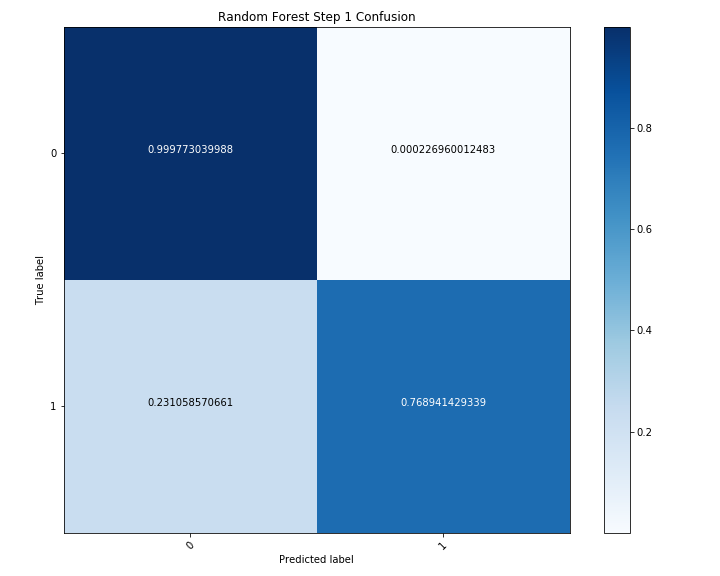
\includegraphics[scale=0.2]{/Users/derekjones2025/workspace/protein_binding/results/full_kinase_set/random_forest_step1_confusion.png}
%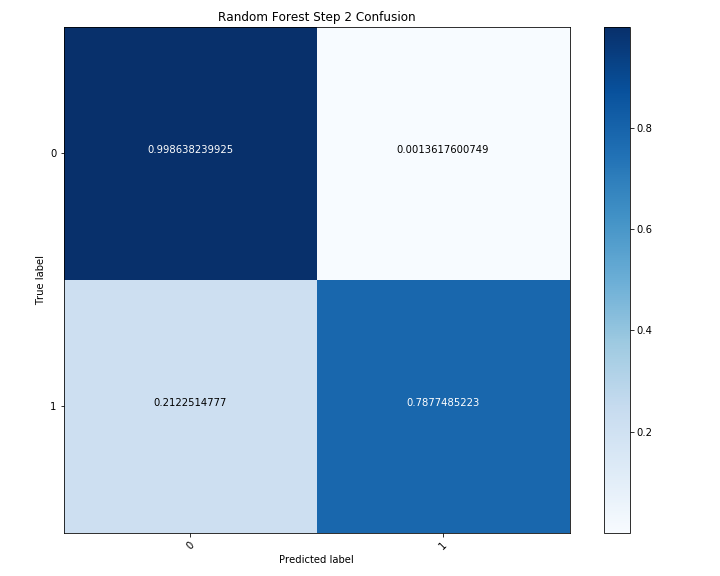
\includegraphics[scale=0.2]{/Users/derekjones2025/workspace/protein_binding/results/full_kinase_set/random_forest_step2_confusion.png}
%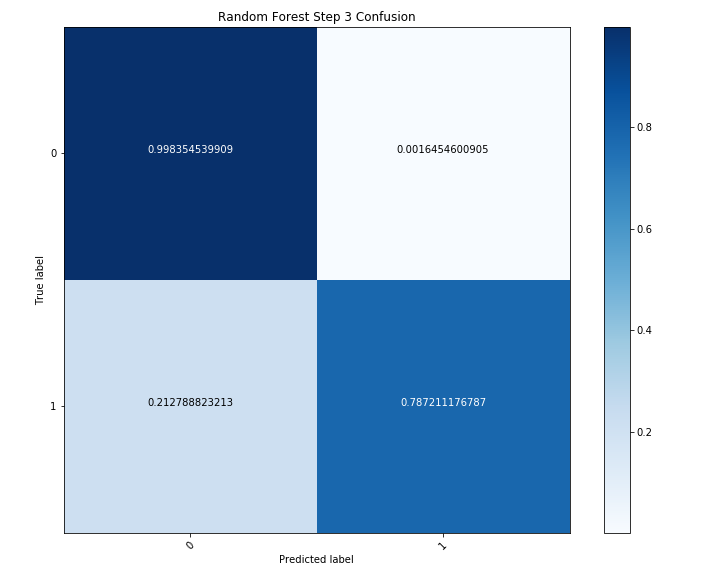
\includegraphics[scale=0.2]{/Users/derekjones2025/workspace/protein_binding/results/full_kinase_set/random_forest_step3_confusion.png}
%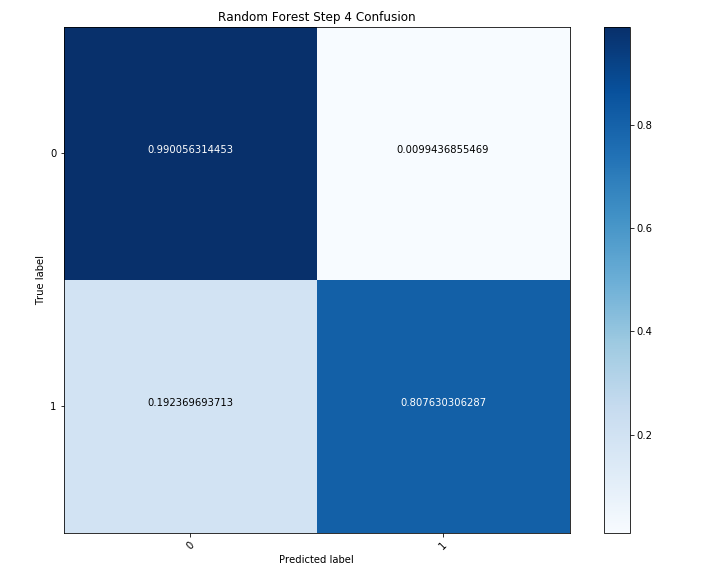
\includegraphics[scale=0.2]{/Users/derekjones2025/workspace/protein_binding/results/full_kinase_set/random_forest_step4_confusion.png}
\end{document}